\section{Ricerca dell'involucro convesso}\label{rircerca-dellinvolucro-convesso}

Si ha un insieme di punti e si vuole trovare il più piccolo involucro convesso che li contiene tutti.

\subsection{Algoritmo di Graham}\label{algortimo-di-graham}

Se l'insieme \emph{Q} contiene \emph{n} punti riesce a risolvere il problema in $O(n \log n)$.

L'algoritmo inizia cercando il punto $p_0$ più in basso. 
Se ci sono più punti con la stessa \emph{y} minima, effettua il tie-breaking prendendo quello più a sinistra.

Dopodiché ordina i restanti $n-1$ punti per angolo polare rispetto a $p_0$ e se due punti hanno lo stesso angolo polare li ordina per distanza crescente da $p_0$

Una volta stabilito l'ordinamento dei punti $p_0, p_1 \ldots, p_{n-1}$, l'algoritmo inizia a costruire incrementante l'involucro convesso utilizzando una struttura dati \emph{S} che si comporta come una pila.

Su \emph{S} è possibile eseguire:

\begin{itemize}
\item
  \textsc{Push($S,p$)}: aggiunge il punto \emph{p} in cima alla pila
\item
  \textsc{Pop($S$)}: elimina il primo elemento della pila
\item
  \textsc{Top($S$)}: restituisce, senza eliminarlo, il valore del primo
  elemento della pila
\item
  \textsc{Next-To-Top($S$)}: restituisce il valore del penultimo elemento
  della pila.
\end{itemize}

L'algoritmo inizia inserendo $p_0$ nella pila, $p_0$ è sicuramente un punto dell'involucro convesso perché è quello più in basso a sinistra. 
Quindi quando c'è solo $p_0$ in \emph{S} si ha l'involucro convesso degenere e per come è stato scelto $ p_0 $ i segmenti $ \overrightarrow{p_0p_1} $ e $\overrightarrow{p_0p_{n-1}}$ non possono essere allineati orizzontalmente e in senso opposto.

Dopodiché per ogni punto restante l'algoritmo prova ad aggiungerlo nel poligono convesso. 
Quando viene aggiunto un nuovo punto viene fatto un controllo per rimuovere da \emph{S} i punti che sono interni.

Questo viene fatto considerando i primi due punti della pila, \emph{p} e \emph{q}, e il punto corrente $p_i$.

Da notare che se nella pila c'è un solo elemento, il punto $p_i$ viene aggiunto senza problemi, perché in quel momento non può essere interno.

Se nel passare dal segmento $\overrightarrow{qp}$ al segmento $\overrightarrow{pp_i}$ c'è una svolta a destra, vuol dire che aggiungendo il punto $p_i$ al poligono, il punto \emph{p} diventa interno e quindi deve essere tolto.

Una volta tolto \emph{p} è necessario ri-effettuare lo stesso controllo perché può essere che anche \emph{q} diventi un punto interno del poligono.

Costruendo il poligono in questo modo si ottiene un poligono semplice perché i vertici vengono scelti in ordine crescente di angolo polare rispetto a $ p_0 $ ed è convesso in quanto passando per ogni vertice si gira sempre a sinistra.

\begin{breakablealgorithm}
	\caption{\textsc{Graham-Scan}: algoritmo per la costruzione dell'involucro convesso}
	\begin{algorithmic}[1]
		\Function{Graham-Scan}{$Q$}
		\State // cerca $p_0$
		\State // ordina $p_1, \ldots, p{n-1}$ per angolo polare rispetto a $p_0$
		\State \textsc{Push}$(S,p_0)$
		\For{$i = 1 \textbf{ to } n-1$}
		    \State $p \gets \textsc{Top}(S)$
		    \State $q \gets \textsc{Next-To-Top}(S)$
		     \While{$q \neq \textsc{Nil} \textbf{ and } \textsc{Turn-left}(q,p,p_i)$}
		        \State \textsc{Pop}$(S)$
		        \State $p \gets q$
		        \State $q \gets \textsc{Next-To-Top}(S)$
		     \EndWhile
		     \State \textsc{Push}$(S,p_i)$
		\EndFor
		\State \Return $S$
		\EndFunction
   	\end{algorithmic}
\end{breakablealgorithm}

Per dimostrare la \textbf{correttezza} dell'algoritmo è necessario dimostrare che un punto viene tolto dal poligono solo quando non appartiene al poligono.

Quando viene eliminato il punto $ q_k $ che si trova in cima alla pila, si ha che questo viene fatto perché in esso o si gira a destra o si prosegue dritto.

Se si gira a destra, tale punto è sicuramente contenuto nel triangolo di vertici $p_0, q_{k-1} \text{ e } p_i$ e quindi è interno al poligono convesso, mentre se si prosegue dritto vuol dire che il punto è interno al segmento $\overline{q_{k_1}p_i}$ e anche in questo caso non appartiene al poligono convesso.


\begin{figure}[htbp]
\centering
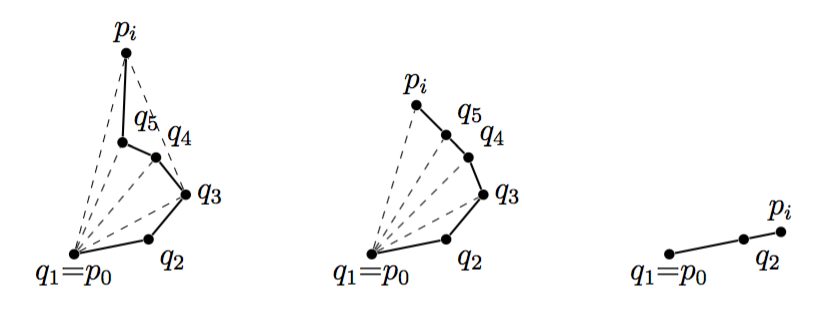
\includegraphics[width=.8\textwidth]{./notes/immagini/l32-fig1.png}
\caption{A sinistra: l'aggiunta del punto $p_i$ porta ad effettuare una svolta a destra sia in $q_5$ che in $ q_4 $, i quali devono essere rimossi dal poligono convesso. Al centro: viene rimosso solamente $ q_5 $ perché appartiene al segmento $\overline{q_4p_i}$. A destra: caso analogo, viene rimosso $q_2$.}
\end{figure}

La \textbf{complessità} dell'algoritmo ha un $O(n)$ per la ricerca di $p_0$, $O(n \log n)$ per l'ordinamento dei punti e un restante $O(n)$ per l'esecuzione del \texttt{for}. 
La complessità totale è quindi dominata da quella della ricerca.

\subsection{Algoritmo di Jarvis}\label{algoritmo-di-jarvis}

L'algoritmo di Jarvis calcola l'involucro convesso in tempo $O(nh)$ dove \emph{h} è il numero di vertici.

L'idea alla base dell'algoritmo è quella di andare a \emph{recintare dei chiodi piantati su un pezzo di legno con uno spago legato ad un punto del poligono convesso}.

L'algoritmo cerca quindi il punto $p_0$ in modo analogo all'algoritmo di Graham, dopodiché cerca tra i restanti punti il punto $q_1$ che ha l'angolo polare più piccolo rispetto al punto di origine $p_0$. 
Una volta trovato questo punto, la procedura viene ripetuta utilizzando come riferimento $q_1$ e così via. 

Quando viene raggiunto il punto più alto del poligono, la semiretta di riferimento viene girata in modo da avere sempre angoli minori di 180°. 
Questo punto viene chiamato $p_t$ ed è quello più in alto, tie-breaking scegliendo quello più a destra.

L'algoritmo termina quando si ritorna al punto di partenza.

\begin{breakablealgorithm}
	\caption{\textsc{Jarvis}: algoritmo per la costruzione dell'involucro convesso}
	\begin{algorithmic}[1]
			\Function{Jarvis}{$Q$}
			    \State // Cerca $p_0$ e $p_t$
			    \State $H[1] \gets p_0$ \Comment{Array che contiene i punti dell'involucro}
			    \State $k \gets 1$
			    \While{$H[k]\neq p_t$}
			        \State $q \gets \text{ Min-Polar-Right}(H[k],Q)$ \Comment{Angolo rispetto la semi-retta destra}
			        \State $k \gets k +1$
			        \State $H[k] \gets q$
			    \EndWhile
			    \State $q \gets \textsc{ Min-Polar-Left}(H[k],Q)$
			    \While{$q \neq p_0$}
			        \State $k \gets k+1$
			        \State $H[k] \gets q$
			        \State $q \gets \textsc{Min-Polar-Left}(H[k],Q)$
			    \EndWhile
			    \State \Return $H$
			\EndFunction
	\end{algorithmic}
\end{breakablealgorithm}

Se la ricerca del minimo angolo polare richiede tempo $O(n)$ si ha che questa viene ripetuta per ogni vertice del poligono e quindi si ha $O(nh)$.

Da notare che si può ottenere un leggero miglioramento andando a rimuovere da \emph{Q} i punti che sono stati aggiunti a \emph{H}.

\subsection{Tecnica incrementale per il poligono convesso}\label{tecnica-incrementale-per-il-poligono-convesso-es-14}

\textbf{\textit{Esercizio 14}} \todo{Verificare correttezza}

Vengono ordinati i punti dell'insieme \emph{Q} da sinistra verso destra, per poi iniziare ad aggiungerli uno ad uno al poligono convesso, il quale inizialmente è composto dal punto più a sinistra.

Per memorizzare i punti del poligono vengono utilizzate due pile, una per i punti della parte bassa e una per i punti della parte alta.

Per ogni nuovo punto che arriva lo si aggiunge alla pila della parte bassa se si trova sotto il punto di partenza o nella pila della parte alta se si trova sopra. L'aggiunta viene fatta in modo analogo a quella dell'algoritmo di Graham in modo da garantire che la pila sulla quale è stato inserito rappresenti ancora un poligono convesso.

Una volta inserito nella pila rimane da controllare che la congiunzione delle due pile sia ancora un poligono convesso e questo viene fatto controllando l'angolo che c'è tra il punto $p_i$ appena inserito in cima alla pila e i due punti che si trovano in cima all'altra pila. Se il punto in cima all'altra pila risulta essere interno al poligono questo viene tolto e viene ripetuto il test fino a che non si ottiene un'involucro convesso.

La complessità è la stessa dell'algoritmo di Graham, perché viene dominata dall'ordinamento dei punti, dato che i test vengono effettuati al massimo $n$ controlli (una volta tolto il punto da una pila questo non ci rientra più).

\subsection{Tecnica divide et impera}\label{tecnica-divide-et-impera-es-15}

\textbf{\textit{Esercizio 15}}\todo{completare}

Vengono ordinati i punti da sinistra a destra e poi vengono divisi in due sotto-insiemi in modo che ognuno contenga la metà dei punti. 
Viene poi cercato il poligono convesso in modo ricorsivo per ognuno dei sue sotto-insiemi.

\ldots{}

\section{Localizzazione dei punti nel piano}\label{localizzazione-dei-punti-nel-piano}

Data una suddivisione in regioni del piano, si vuole trovare una struttura dati che permetta di trovare rapidamente a quale regione del piano appartiene un dato punto. 
Le regioni possono anche avere area infinita e non necessariamente convesse.

Queste regioni vengono rappresentate da una successione di lati e vertici che formano il poligono in senso antiorario.

Il problema può però essere ridotto alla ricerca del segmento dominante, ovvero dati \emph{n} segmenti ed un punto \emph{p}, trovare il segmento $s_i$ che si trova immediatamente sopra al punto \emph{p}.

Risolvere questo problema permette di risolvere il problema della localizzazione utilizzando tutti i lati delle regioni e associando ad ogni lato l'informazione relativa a quale regione si trova sotto.

Se una regione è illimitata si può utilizzare un bordo, ma all'inizio ci limiteremo al caso senza regioni illimitate.

\subsection{Segmento dominante}\label{segmento-dominante}

Ci sono $s_1,  \ldots s_n$ segmenti e un punto \emph{p}, volgiamo trovare quale segmento si trova immediatamente sopra a \emph{p}, assumendo che non ci siano segmenti verticali o segmenti che si intersecano e che ci sia almeno un segmento sopra il punto \emph{p}.

Queste restrizioni sono presenti solo per semplificare l'algoritmo, ma possono essere rimosse, ad esempio spezzando i segmenti che si intersecano.

Come prima cosa viene definita una regione $R_0$ che contiene tutto il piano. Dopodiché utilizziamo $s_1$ per suddividere $R_0$ nelle 4 regioni $R_1, \ldots R_4$ come riportato in figura.

\begin{figure}[htbp]
\centering
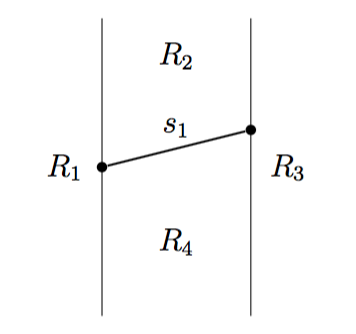
\includegraphics[width=.2\textwidth]{./notes/immagini/l32-fig2.png}
\caption{Suddivisione di $R_0$}
\end{figure}
\FloatBarrier

Dopodiché viene preso in considerazione il segmento successivo $s_2$ e lo utilizziamo per dividere ulteriormente il piano in regioni.

\begin{figure}[htbp]
\centering
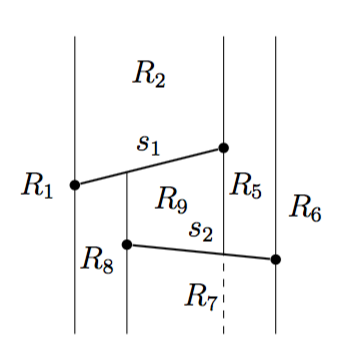
\includegraphics[width=.2\textwidth]{./notes/immagini/l32-fig3.png}
\caption{Suddivisione con $s_2$, $R_7$ è a cavallo di $R_3$ e $R_4$}
\end{figure}

Da notare che se due parti sono limitate superiormente dallo stesso segmento, vengono unite in un'unica parte.

Il partizionamento del piano può essere schematizzato in un DAG. 
Il grafo ottenuto non è un albero, per il fatto che più parti possono essere unite in un unica parte.

\begin{figure}[htbp]
\centering
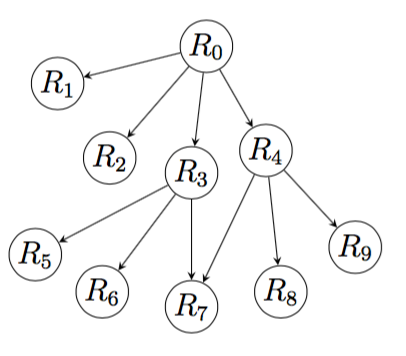
\includegraphics[width=.2\textwidth]{./notes/immagini/l32-fig4.png}
\caption{DAG rappresentate la suddivisione del piano}
\end{figure}

Una volta suddiviso il piano utilizzando tutti i segmenti si ottiene un DAG le cui \emph{``foglie''} rappresentano le regioni del piano e ogni nodo ha al massimo 4 nodi adiacenti.

Una volta costruito il grafo si parte da $R_0$ e ci si sposta sulla regione adiacente al nodo relativo a $R_0$ e che contiene il punto \emph{p}.

Per verificare se un punto si trova all'interno di una data regione, come prima cosa si valuta se la \emph{x} del punto si trova tra $x_1$ e $x_2$, ovvero le rette verticali che delimitano la regione. 
Se il punto si trova tra le due rette, viene verificato con \textsc{Angle-Left} se si trova sopra il segmento $s_1$ inferiore della regione e sotto il segmento $s_2$ superiore della regione.

Si ha quindi che il test di appartenenza ad una regione può essere fatto in tempo costante e deve essere ripetuto per ogni regione fino all'arrivo in una foglia. 
Nel caso peggiore si ha quindi una complessità $O(n)$.
\FloatBarrier
\subsubsection{Randomizzazione}\label{randomizzazione}

L'ordine in cui si valutano i segmenti influisce sul partizionamento che si ottiene, il quale a sua volta influisce sulla lunghezza dei cammino del DAG.

Il cammino che congiunge il nodo $R_0$ con le varie foglie rappresenta la storia di una regione e la lunghezza del cammino che porta ad una certa regione $R$ viene detta \textbf{lunghezza della storia della regione} $R$ ed è proporzionale al numero di volte che la regione viene modificata durante la costruzione del grafo.

Assumiamo quindi che l'ordine di valutazione dei segmenti $s_1, \ldots, s_n$ sia casuale e ci chiediamo quale sia la lunghezza media della storia della regione \emph{R} che contiene il punto \emph{p}.

Per ragionare sulla storia si può procedere a ritroso, ovvero partendo dal partizionamento completo si possono via via togliere i segmenti aggiunti per ultimi.

Supponendo che siano stati rimossi i segmenti $s_{i+1}, \ldots, s_n$, il punto \textit{p} apparterrà ad una certa regione $ R $, la quale, quando verrà rimosso il segmento $s_i$, cambierà solo se il segmento $ s_i $ la delimita e per come sono definite le regioni, ci sono 4 modi in cui un segmento può delimitare una regione (sopra, sotto, estremo destro, estremo sinistro).

Siccome il segmento $s_i$ viene scelto a caso tra quelli ancora da rimuovere, la probabilità che la regione $ R $ cambi è di $ 4/i $.

Il valore atteso di questa distribuzione risulta essere

$$
\sum\limits_{i=1}^{n} \frac{4}{i} = O(\log n)
$$

Pertanto lunghezza media della storia di una regione è $ O(\log n) $ e quindi il tempo medio per la ricerca della regione di appartenenza di un punto è $ O(\log n) $.